% !TEX root=./report.tex

\section{Evaluation}

We assure the correctness and quantify the visual improvements resulting from the algorithms by an empirical study on the video streams of the highway cameras.

\subsection{Study objects}
\begin{figure}[t]
    \begin{center}
    % \fbox{\rule{0pt}{2in} \rule{0.9\linewidth}{0pt}}
       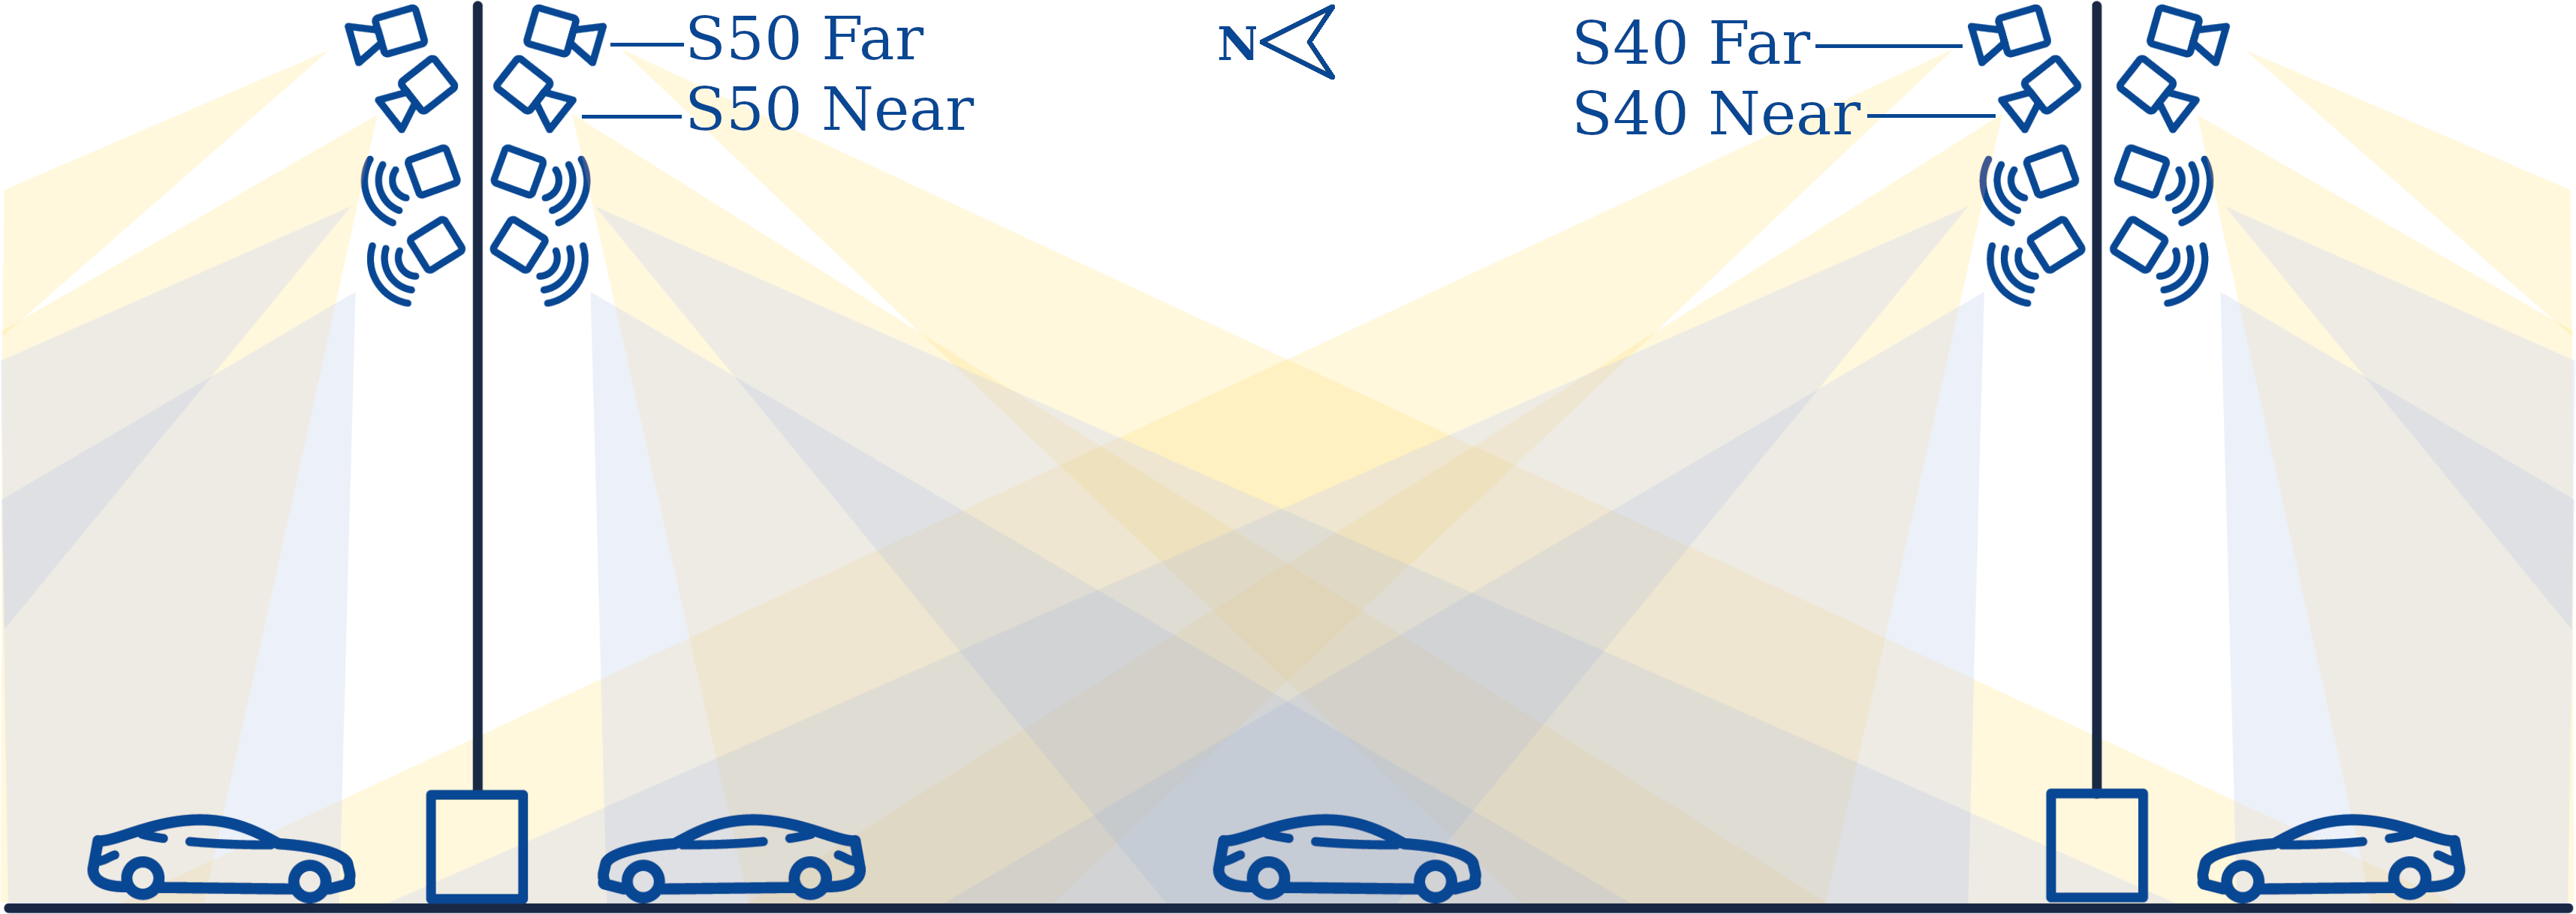
\includegraphics[width=\linewidth]{images/cameras_schema.png}
    \end{center}
       \caption{The schematic camera setup along the highway A9.
       The cameras \camsf{4} and \camsn{4} are facing north,
       the cameras \camsf{5} and \camsn{5} are facing south.}
    \label{fig:cameras_schema}
    \end{figure}

We use video recordings from the four cameras mounted to the two gantry bridges internally named S40 and S50. The schematic camera setup is displayed in \autoref{fig:cameras_schema}.

The dataset consists of four recordings, each with of a length of $1495$ frames over $\sim 60$ seconds at $25$ frames per second.

The recordings are taken on a day with strong winds to ensure high jitter in the video feed to optimally test the Dynamic Stabilization algorithm described in \autoref{sec:dynamic_stabilization}. 

\subsection{Dynamic stabilization}
To evaluate the Dynamic Stabilization algorithm described in \autoref{sec:dynamic_stabilization} we have come up with two metrics to quantify the environmental influences.

\subsubsection{Optical Flow}
\begin{figure*}[!ht]
    \centering
    \begin{tabular}{cc}
      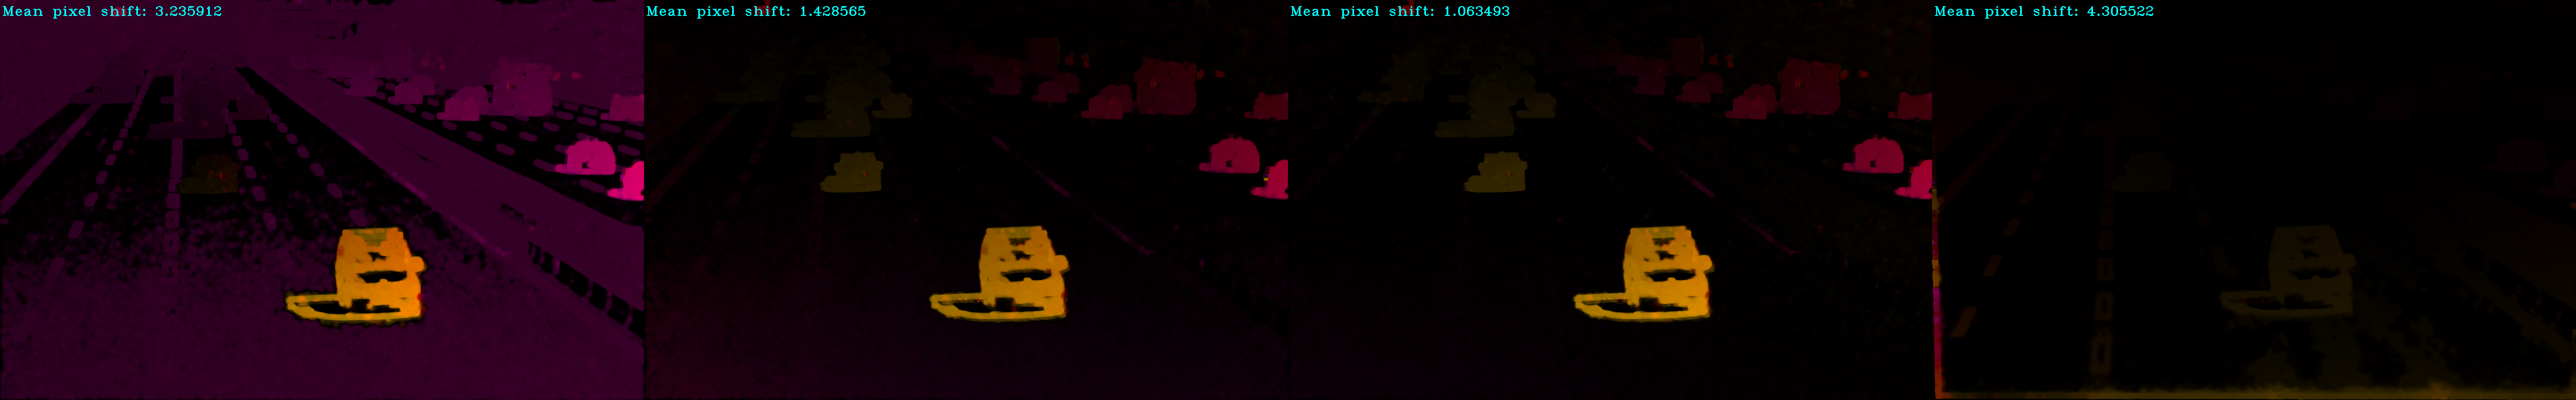
\includegraphics[width=0.95\linewidth]{images/frame_1317_cropped.png}    &  
    \end{tabular}
    \caption{
        The dense Optical Flow displaying the pixel displacement.
        The lighter the color the further the displacement. 
        The angle of displacement is color coded according to the HSV color circle.  
        From left to right: Original frame, 
        stabilized using SURF \cite{bay10.1007/11744023_32,opencv_library} feature detector,
        ORB \cite{rublee6126544, opencv_library} feature detector and
        FAST \cite{Ghahremani_2021,opencv_library} feature detector with FREAK \cite{alahi6247715,opencv_library} feature descriptors.
        In the original frame the violet background color indicates a jittery camera movement. 
        The car in the lower half is driving in the opposite direction as the camera jitters. 
    }
    \label{fig:optical_flow_example}
\end{figure*}

The Optical Flow describes the apparent motion of image objects between two consecutive frames. 
It is a 2D vector field where each vector is a displacement vector showing the movement of points between the frames caused by movement of the objects or cameras.

We use the dense Optical Flow estimation algorithm proposed by Farnebäck \cite{farnback10.1007/3-540-45103-X_50,opencv_library} to measure the displacement of each pixel between the frames. 
We calculate the mean displacement over the whole image to get the overall displacement. 
\autoref{fig:optical_flow_example} shows one frame of Optical Flow calculated.

We see that the dynamically stabilized video feed exhibit a substantially lower mean displacement between frames as the displacement from camera jitter is removed.
This leaves us with only the expected displacement resulting from moving objects, \eg{} vehicles on the highway or shaking trees.

\begin{figure*}[!ht]
    \centering
    \begin{tabular}{cc}
      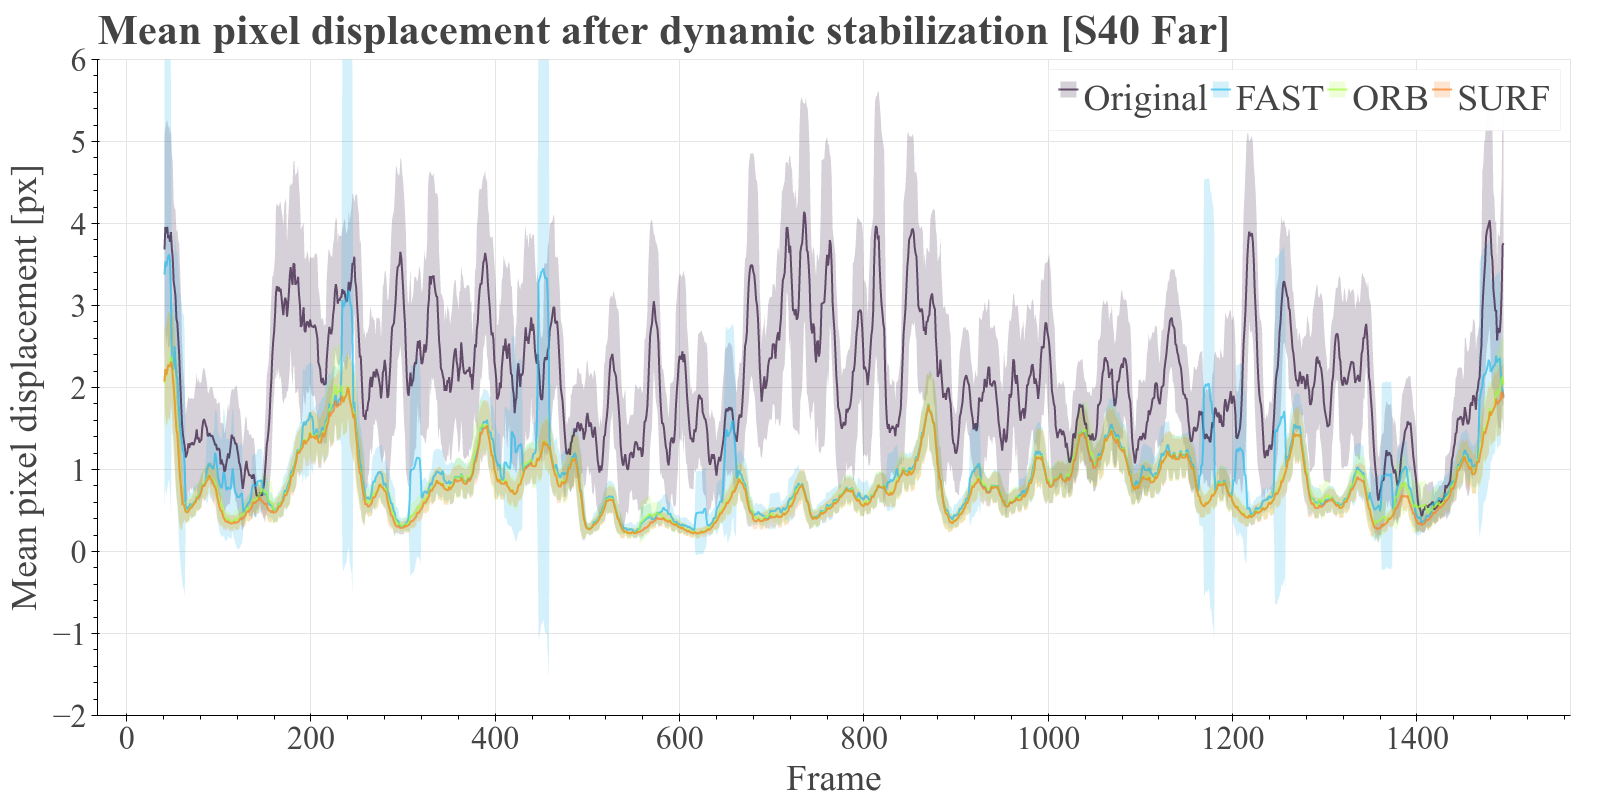
\includegraphics[width=0.475\linewidth]{diagrams/mean_pixel_shifts_after_dynamic_stabilization_s40_far.png}    &  
      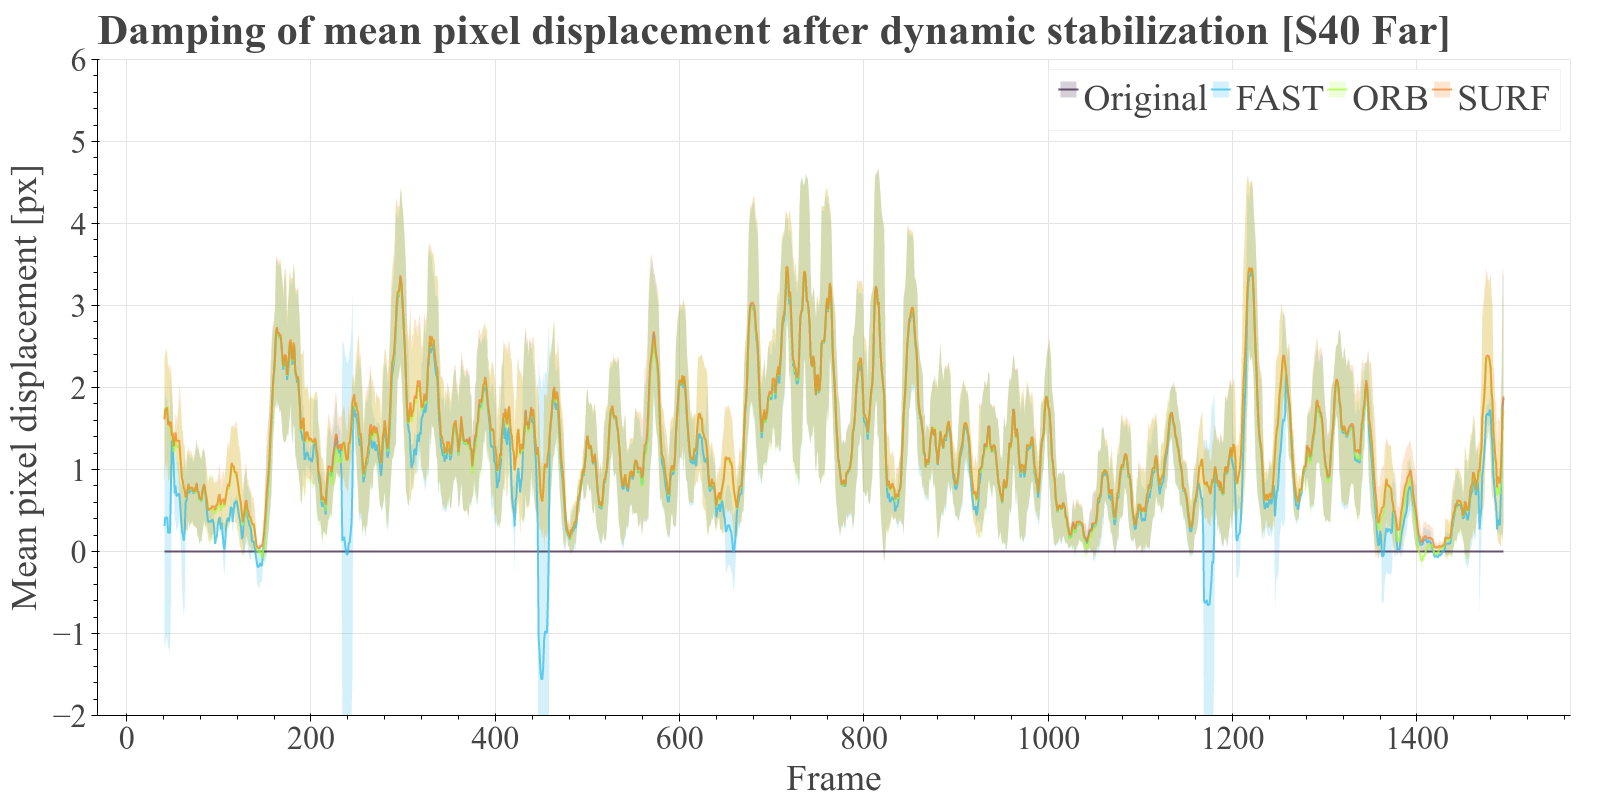
\includegraphics[width=0.475\linewidth]{diagrams/damping_mean_pixel_shifts_after_dynamic_stabilization_s40_far.png}    
\end{tabular}
    \caption{Left: 
        Comparison of the three implemented dynamic stabilizers and the original not stabilized video feed using Optical Flow as metric (lower is better).
        The stabilizers are based on the 
        FAST \cite{Ghahremani_2021,opencv_library} feature detector with FREAK \cite{alahi6247715,opencv_library} feature descriptors,
        SURF \cite{bay10.1007/11744023_32,opencv_library} feature detector and
        ORB \cite{rublee6126544, opencv_library} feature detector.
        The graphs display the mean pixel shift at each frame. 
        Right: 
        The damping capabilities of the same three stabilizers (higher is better). 
        The graphs approximate the removed jitter in the mean pixel shift between the original video and the stabilizer at each frame.\\
        For visualization the values are filtered using the rolling mean over 12 frames. 
        The light areas display the standard deviation within the window.
    }
    \label{fig:dynamic_stabilization_s40_far}
\end{figure*}

\autoref{fig:dynamic_stabilization_s40_far} displays the mean pixel displacement per frame.
It shows that the displacement with especially the SURF \cite{bay10.1007/11744023_32,opencv_library} feature detector is lowered greatly. 
The damping approximates the removed jitter and also displays a huge lowering in mean displacement.


\begin{figure}[!ht]
      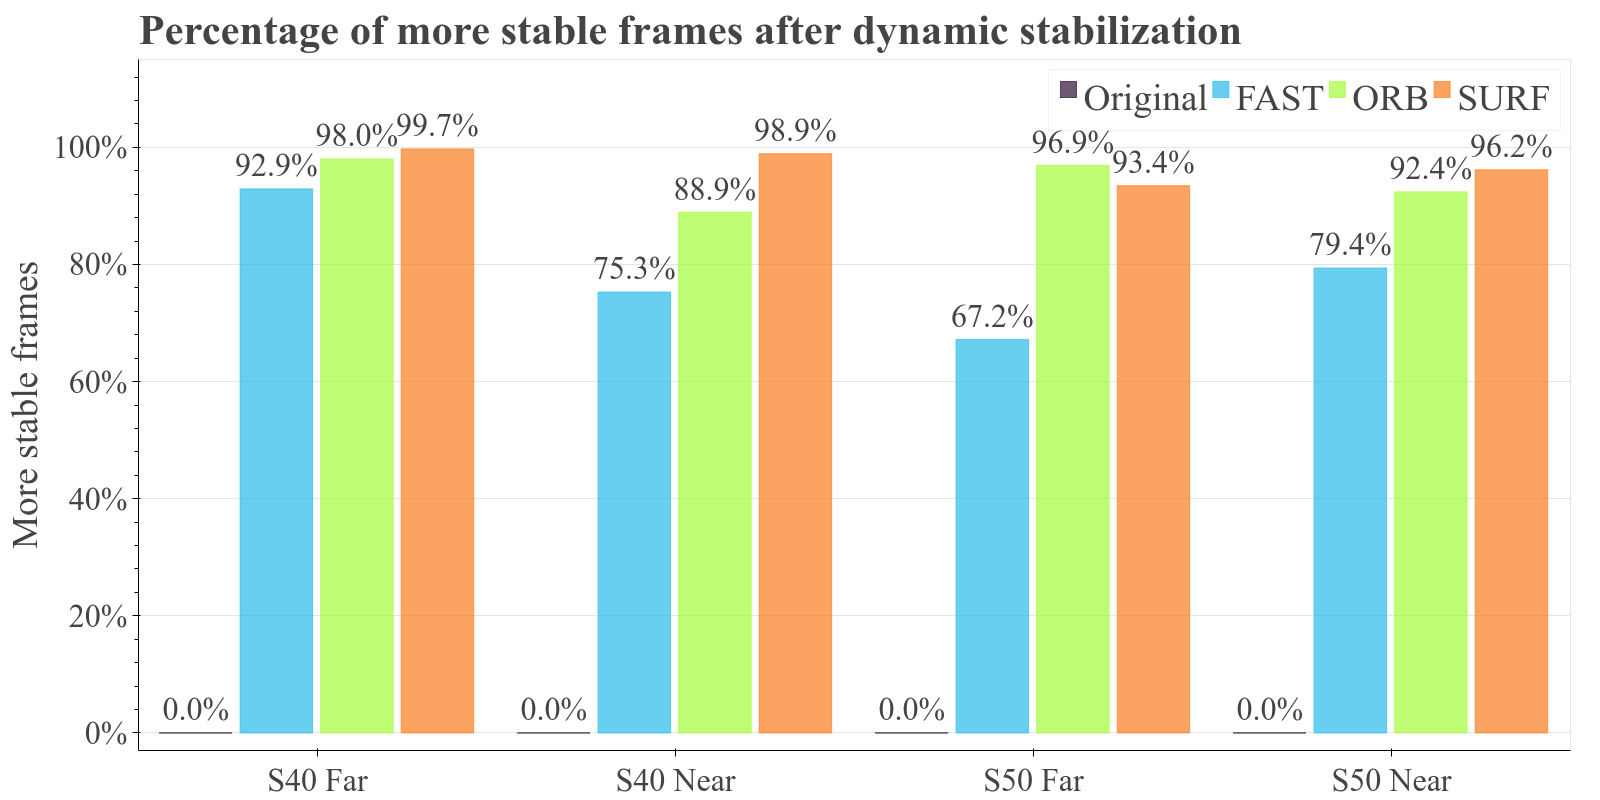
\includegraphics[width=\linewidth]{diagrams/stats.png}    
    \caption{
        Comparison of the percentages of more stable frames after dynamic stabilization per camera and stabilizer.
        A frame is classified as more stable if the mean pixel displacement is lower as in the original video feed. 
        The comparison shows that the stabilizers all improve the video stability, but the SURF \cite{bay10.1007/11744023_32,opencv_library} feature detector based stabilizer outperforms the others.          
    }
    \label{fig:dynamic_stabilization}
\end{figure}

\autoref{fig:dynamic_stabilization} further quantifies the stabilization of the frames.

\paragraph{Problem of Optical Flow as a metric}
Unfortunately, Optical Flow exhibits one major problem as a metric: 
It cannot distinguish between dynamically moving objects and static scene.
This especially introduces a problem when a jitter of the camera moves the pixels in the same direction as the vehicles path is pointing in image space.
By this jitter the movement of the camera blurs the movement of the dynamic objects into the background and thus removes some of the real movement.
This shows some frames after stabilization to be worse than before. 
This should be taken with caution as the Optical Flow cannot detect the relative motion and thus is not a definite measure for the jitter.
Nonetheless it gives a good hint at the overall stabilization capabilities and can become a measure together with the following measure of the path length of a pixel on a dynamic object. 

\subsubsection{Track features and calculate path smoothness}
